\documentclass[11pt]{report}
\usepackage[german, english]{babel}
\usepackage{geometry}                % See geometry.pdf to learn the layout options. There are lots.
\geometry{a4paper}                   % ... or a4paper or a5paper or ... 
%\usepackage[parfill]{parskip}    % Activate to begin paragraphs with an empty line rather than an indent
\usepackage{xifthen}
\usepackage{xstring}			% to check content of strings in xifthen
\usepackage{graphicx}
\usepackage{amssymb}
\usepackage{epstopdf}
\usepackage[utf8]{inputenc}
\usepackage{hyperref}
\usepackage{fancyhdr}
\usepackage{float}

\IfStrEq*{\languagename}{english}
	{
		\newcommand{\dalabel}{Diploma Thesis}
		\newcommand{\submittedlabel}{Submitted by}
		\newcommand{\datelabel}{Date}
		\newcommand{\supervisorlabel}{Supervisor}
		\newcommand{\projectpartnerlabel}{Project Partner}
	}
	{
		\newcommand{\dalabel}{Diplomarbeit}
		\newcommand{\submittedlabel}{Eingereicht von}
		\newcommand{\datelabel}{Datum}
		\newcommand{\supervisorlabel}{Betreuer}
		\newcommand{\projectpartnerlabel}{Projektpartner}
	}
 % This file should really be touched
\newcommand{\titleofthesis}{Visulation of the NoBeard Virtual Machine}
\newcommand{\department}{Informatik} % Replace by your department

\newcommand{\firstauthor}{Egon Manya}
\newcommand{\firstauthorclass}{5AHIF}

\newcommand{\duedateen}{April 4, 2018}
\newcommand{\duedatede}{4. April 2018}
\newcommand{\supervisor}{Peter Bauer}
 % Set basic data (author, title, etc.) of your thesis
\begin{document}
\rhead{
\includegraphics[scale=.9]{images/Logo.png}}
\cfoot{}
\begin{titlepage}
\thispagestyle{fancy}

\begin{center}

\vspace*{8em}

{\LARGE \dalabel}

\vspace{2em}

{\large Höhere Technische Bundeslehranstalt Leonding \\[.5em]
Abteilung für \department}

\vspace{8em}

{\Huge \titleofthesis}
\end{center}

\vspace{18em}

\begin{tabular}{ll}
\ifthenelse{\isundefined{\firstauthor}}{}{\submittedlabel: & {\bf \firstauthor, \firstauthorclass}}
\ifthenelse{\isundefined{\secondauthor}}{}{ \\[.5em] & {\bf \secondauthor, \secondauthorclass}}
\ifthenelse{\isundefined{\thirdauthor}}{}{ \\[.5em] & {\bf \thirdauthor, \thirdauthorclass}}
 \\[.5em]
\datelabel: & {\bf \duedateen} \\[.5em]

\supervisorlabel: & {\bf \supervisor} \\[.5em]

\ifthenelse{\isundefined{\projectpartner}}{}{\projectpartnerlabel: & {\bf \projectpartner}}
\end{tabular}
\end{titlepage}
 % Should not be necessary to touch this file
\section*{Declaration of Academic Honesty}
Hereby, I declare that I have composed the presented paper independently on my own and without any other resources than the ones indicated. All thoughts taken directly or indirectly from external sources are properly denoted as such.

This paper has neither been previously submitted to another authority nor has it been published yet. \\[1em]
Leonding, \duedateen \\[5em]
\ifthenelse{\isundefined{\firstauthor}}{}{\firstauthor}
\ifthenelse{\isundefined{\secondauthor}}{}{\kern-1ex, \secondauthor}
\ifthenelse{\isundefined{\thirdauthor}}{}{\kern-1ex, \thirdauthor} \\[5em]

\begin{otherlanguage}{german}
\section*{Eidesstattliche Erklärung}
Hiermit erkläre ich an Eides statt, dass ich die vorgelegte Diplomarbeit selbstständig und ohne Benutzung anderer als der angegebenen Hilfsmittel angefertigt habe. Gedanken, die aus fremden Quellen direkt oder indirekt übernommen wurden, sind als solche gekennzeichnet.

Die Arbeit wurde bisher in gleicher oder ähnlicher Weise keiner anderen Prüfungsbehörde vorgelegt und auch noch nicht veröffentlicht. \\[1em]
Leonding, am \duedatede \\[5em]
\ifthenelse{\isundefined{\firstauthor}}{}{\firstauthor}
\ifthenelse{\isundefined{\secondauthor}}{}{\kern-1ex, \secondauthor}
\ifthenelse{\isundefined{\thirdauthor}}{}{\kern-1ex, \thirdauthor} \\[5em]
\end{otherlanguage}

\begin{abstract}
The target of this diploma thesis is to extend an available system programming environment which is called the NoBeard project. The project is developed to enable students to gain some experiences in the field of system programming by coding on assembler level with basic instructions. In addition, the reader of this thesis gets a basic knowledge about formal languages and their uses.

Initially, the project contained three main components:
\begin{itemize}
\item {\em The NoBeard Machine:} A stack based virtual machine with a small set of instructions. The main task of the machine is to execute NoBeard object files.
\item {\em The NoBeard Assembler:} Provided to write programs for the NoBeard Machine.
\item {\em The NoBeard Compiler:} Includes a dedicated programming language and the corresponding compiler to simplify the writing of codes for the NoBeard Machine.
\end{itemize}

The purpose of this thesis was to develop a proper concept of a graphical user interface for the virtual machine.
The concept has to focus the didactic aims to enable users to explore the execution cycle of an assembler instruction, the execution of programs on assembler level, the monitoring of stack frames, the expression stack etc\ldots 

Furthermore, the system is extended with some debugger functions such as setting break points, stepping on assembler instruction level etc\ldots

The initial version of the NoBeard project was developed in Java, therefore the graphical user interface had to be implemented with the Java FX framework.
Primary, it was conceived with the NetBeans IDE on the ant build system, however the entire project was migrated to Maven and further developed using the IntelliJ IDEA environment.
\end{abstract}

\begin{otherlanguage}{german}
\begin{abstract}
Das Ziel dieser Diplomarbeit ist es, eine verfügbare Systemprogrammierumgebung zu erweitern, die als NoBeard-Projekt bezeichnet wird. Das Projekt wurde entwickelt, um den Studierenden zu ermöglichen, einige Erfahrungen im Bereich der Systemprogrammierung zu sammeln, indem sie auf Assembler-Ebene mit grundlegenden Anweisungen kodieren. Darüber hinaus erhält der Leser dieser Arbeit ein grundlegendes Wissen über formale Sprachen und ihre Verwendung.

Ursprünglich enthielt bestand das Projekt aus drei Hauptkomponenten:
\begin{itemize}
\item {\em Die NoBeard Maschine:} Eine stack-basierte virtuelle Maschine mit einer kleinen Menge von Anweisungen. Die Hauptaufgabe der Maschine besteht darin, NoBeard-Objektdateien auszuführen.
\item {\em Der NoBeard Assembler:} Zum Schreiben von Programmen für die NoBeard Maschine.
\item {\em Der NoBeard Compiler:} Enthält eine spezielle Programmiersprache und den entsprechenden Compiler, um das Schreiben von Codes für die NoBeard Maschine zu vereinfachen.
\end{itemize}

Der Zweck dieser Arbeit war es, ein geeignetes Konzept für eine grafische Benutzeroberfläche für die virtuelle Maschine zu entwickeln.
Das Konzept muss die didaktischen Ziele fokussieren, um Benutzern zu ermöglichen, den Ausführungszyklus eines Assemblerbefehl zu erkunden, die Ausführung von Programmen auf Assembler-Ebene, die Überwachung von Stack-Frames etc\ldots

Darüber hinaus wurde das System um einige Debugger-Funktionen, wie das Setzen von Breakpoints, erweitert

Die ursprüngliche Version des NoBeard-Projekts wurde in Java entwickelt, daher musste die grafische Benutzeroberfläche mit dem Java FX-Framework implementiert werden.
Primär wurde es mit der NetBeans-IDE auf dem ant-Build-System konzipiert, jedoch wurde das gesamte Projekt auf Maven migriert und unter Verwendung der IntelliJ IDEA-Umgebung weiterentwickelt.

\end{abstract}
\end{otherlanguage}
 % Declaration of Academic Honesty, Abstracts, Acknowledgments, 
\tableofcontents
\chapter{Introduction}
\section{Initial Situation}
The NoBeard environment is developed to support the courses of Theoretical Informatics conducted for third grade students of the Department of Informatics at the HTBLA Leonding. The project was introduced by Prof. DI Peter Bauer with the purpose that students get the possibility to gain some experience in the field of system programming. 

The NoBeard tools consists of a stack based virtual machine, an assembler and a basic compiler with the corresponding language. The components here are developed in the simplest way  to facilitate the operation of the user as much as possible.

\section{Goals}
The general goal of this thesis was to extend the already existing NoBeard project by a graphical user interface to make the use of the virtual machine more simple. It was the highest priority to meet all the usability requirements. Amongst other things, it includes a better and easier use of the virtual machine compared to command line interfaces. Through the advantages of a GUI users are able to get a better overview of an assembler program execution and its data memory state.

The other major goal of this continuation project was the introducing of a debugger into this system. This tool need to cover nearly all basic debugger functionalities for assembler programs such as toggling breakpoints or stepping through assembler instruction. Of course, the concept should support as well CLI as GUI devices.

\section{Structure of the Thesis}
\subsection{Formal Languages}
This chapter is intended to provide a rough overview of formal languages, their structure (grammars), and usefulness. It gives a short description about the syntax of a language.

\chapter{Formal languages \& Compiler construction}
\chapter{Description of the GUI}
\paragraph{This chapter describes how to use the graphical user interface of the NoBeard virtual machine and serves at the same time as a user manual. The application is developed as simple as possible to use. With the three main tools the user can load and run NoBeard object files, debugging running programs and get a whole view of the data memory.}
\begin{center}
	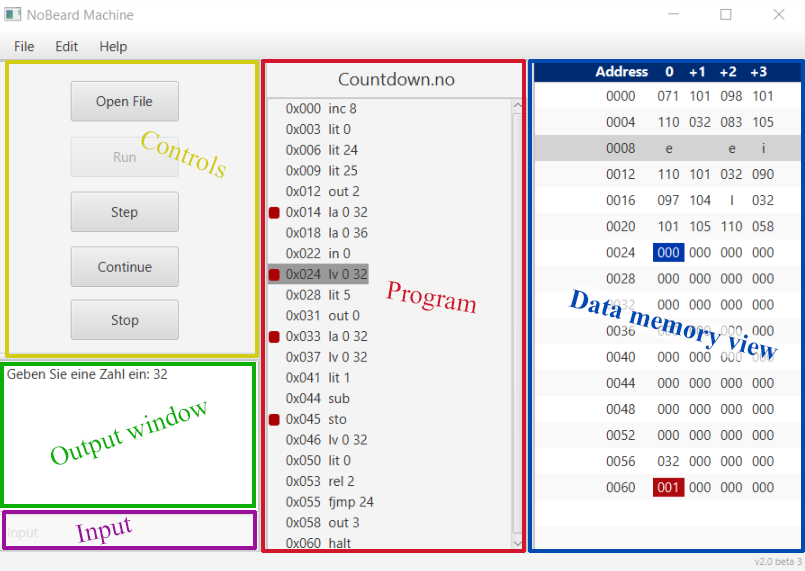
\includegraphics[scale=.90]{images/screenshot-0.png}
\end{center}
\section{Loading \& Running a program}
\paragraph{By starting the user interface, a NoBeard object file has to be loaded by a click on the “open file” button. Than the user can choose the desired file. Afterward, the window shows the content and the title of the opened program which is now executable.}

\paragraph{The content lists instructions with the belonging addresses and operators. By hitting the “Run” button, the machine executes the loaded program. Under the control buttons there is a window which simulates a terminal where the user can see the outputs of the running program. If the program runs against an input instruction, the machine stops and requests the user for an input which can be done under the output window. To submit an input, the Enter key has to be pressed.}

\begin{figure}[h] 
	\centering
	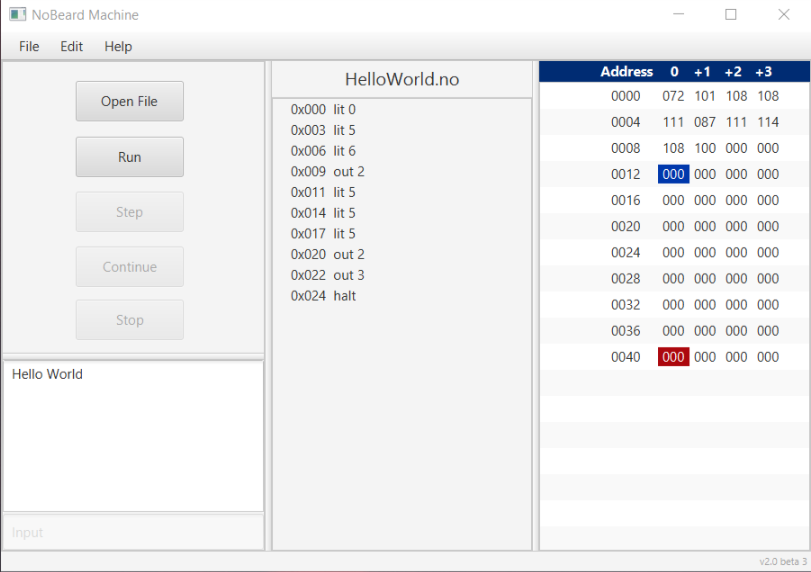
\includegraphics[scale=.75]{images/screenshot-1.png}
	\caption{Executed "Hello World" program}
\end{figure}

\section{Debugging}
\paragraph{To debug a program the user has to set breakpoints. These breakpoints can be placed by clicking on the studied address. If a breakpoint has been placed and the program is about to start, it runs only until the line where the breakpoint has been set.}

\paragraph{Than the user is able to step one line further or jump to the next breakpoint. Stepping is handled by the “Step” button as shown in the following picture. By clicking on the “Continue” button, the program runs from the current line until the next breakpoint. If there is not any breakpoint left from the current line, it runs until the end of file. Optionally, the user is able to stop the program during the execution. This could be achieved by the “Stop” button.}

\begin{figure}[h] 
	\centering
	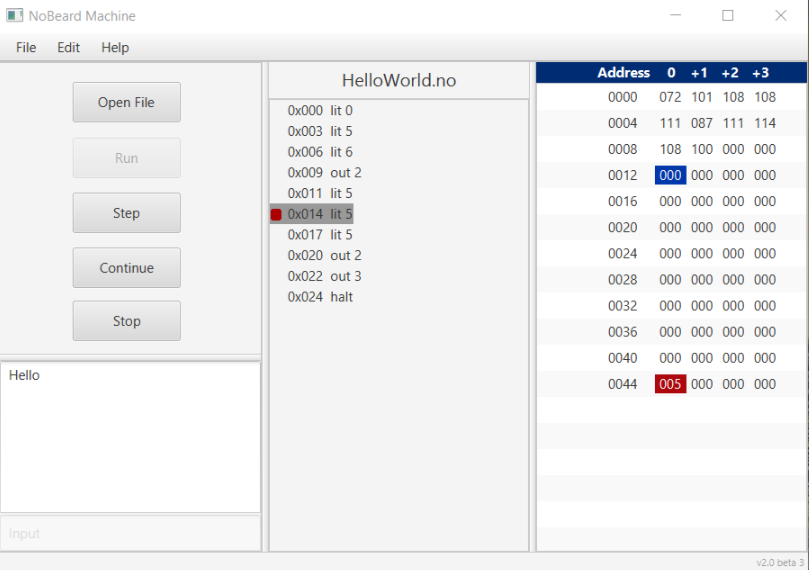
\includegraphics[scale=.75]{images/screenshot-2.png}
	\caption{Debugging the "Hello World" program}
\end{figure}

\section{Data Visualization}
\paragraph{On the right side of the window is the visualisation of the data memory view in a list form. This view lists data byte wise from the data memory of the machine. Each line of the list view has a content of an address given in decimal notation following by four bytes raw data. The memory is separated in two parts. The list starts on the top with the string constants followed by stack frames of the currently running functions. While the frame pointer is highlighted with a blue background, the stack pointer is signed with a red background. The user has also the possibility to convert confused raw data to characters or integers.}
\begin{figure}[h] 
	\centering
	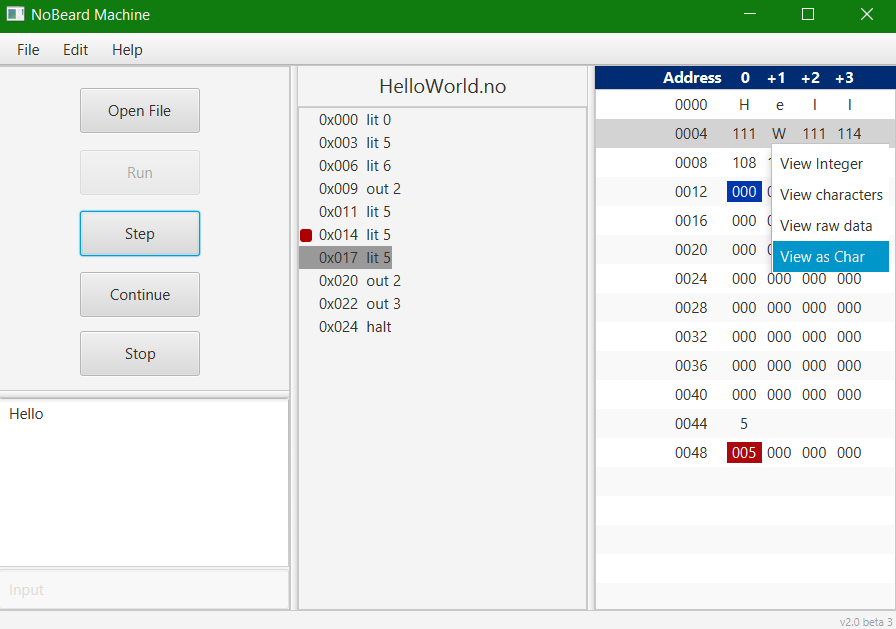
\includegraphics[scale=.60]{images/screenshot-3.png}
	\caption{Converting data to characters}
\end{figure}
\paragraph{With a right click on the selected line of the list, a context menu could be opened. This menu includes following functions: showing integer, characters of the whole line, a single character or converting back the line to raw data. To make the conversion from raw data to alphanumeric characters or integers more easy and fast, a multi selection function is developed for the list of the data memory.}
\chapter{Implementation}
\paragraph{The Implementation of the project is written in Java on the integrated development environment IntelliJ. This IDE is one of the best options for coding because of the huge variety of benefits just like maven. This is a software management and build automation tool which is based on the concept of a project object modem (POM). One of the biggest feature in Maven is the dependency management. Maven automatically downloads in POM file declared libraries and plug-ins from a repository and stores them local. The local repository is a folder structure that is used as a centralized storage place for locally built artifacts and as a cache for downloaded dependencies. The Maven command mvn install builds a project and places its binaries in the local repository. Then other projects can utilize this project by specifying its coordinates in their POMs.}
\paragraph{The NoBeard GUI depends on some existing external package libraries. These libraries include a wide amount off packages. One of the most important package is the “machine”. This is defined as the core of the whole project because it has the most significantly parts including:}
\begin{itemize}
\item \textbf{NoBeardMachine: }a stack based machine with instructions defined as co-operator
\item \textbf{ControllUnit: }is responsible to execute commands and instructions
\item \textbf{DataMemory: }a byte addressed storage
\item \textbf{CallStack: }provide functions to add and remove frames from stack and maintains the expression stack
\item \textbf{InstructionSet: }a list of instructions and their implementations
\end{itemize}
\paragraph{The GUI is designed very similar to the Model-View-Controller pattern. However, this project is not depending on any database so it comes without any Model. The view is a single fxml file which holds the view components of the layout. It was created with an external tool called SceneBuilder that allows developers to design UI without any coding, just drag \& drop with the mouse. Every item of the view has an fx:id which is used in the controller to get easy access to the items. The controller is responsible for the coordination and operation of the view. Initially, it gets an instance of the NoBeard machine where simple program can be executed. The opening of a NoBeard object file is operated with the help of a BinaryFileHandler. After a successful opening of the object file, it has to be disassemble. This function converts binary files to primary program data where addresses, instructions and operands become visible on the UI.}
\paragraph{By finishing the translation, the machine has to load the string storage and the program from the object file. Program data is filled in a VBox with a CheckBox and text of the data for every line. All of the CheckBoxes gets an OnAction event which add and remove breakpoints from the machine.}
\paragraph{On starting a program, a new external thread has to be started where the machine runs separate from the UI. Its executes step by step every instruction of the program until any interruptions. It can be interrupted by a breakpoint, input request or by a halt instruction.}
\section{Interruption by breakpoint (Observer pattern)}
\paragraph{The implementation for the maintaining of breakpoints is coded with a simple observer pattern design to achieve the best performance of the virtual machine. The machine is completely separated from the breakpoint stuff. It runs only until its state equals to “running”. So, a new instruction is introduced, called “BREAK”, which sets the machine in to a “blocked” state. The ControlUnit class is going to be an Observable. Then a new Observer class is implemented which is called debugger that is holding all breakpoints in a HashMap. This HashMap stores the address and the instruction of a breakpoint. The debugger class contains in all three major functions. Adding, removing breakpoints to the HashMap and replacing an instruction at a specified address from the program memory to a new one. The selection of a breakpoint on the UI calls the set or remove function from the debugger, as the case may be. As soon as a breakpoint is selected, it will be stored to the HashMap with its original instruction and at same time replaces the original instruction by the newly added break instruction. This break instruction set the machine to a blocked state and notify the observer to change the break instruction back to the original one which is stored in the HashMap. Now the machine is blocked at a specified breakpoint and the user can take a look to the current stack frames and go one step further in the program or continue the execution cycle to a next breakpoint. However, when the user wants to step further to execute the current instruction where the breakpoint is, a switch back to the break instruction is needed again after the original instruction completed.}
\section{Interruption by input request (Threading)}
\paragraph{As already mentioned, the virtual machine runs on a separate thread so every time the user has to operate an input, a switch to the UI thread is needed. Otherwise it would cause a critical section between the threads. The synchronization of these two threads is implemented with the semaphore construction. The NoBeardMachine contains two interfaces to optimize outputs and inputs on the used device. As soon as the machine executes an input instruction (IN), it calls firstly a function from the input interface either hasNextInt() or hasNext(). Both do the same thing, checks whether there is an input by the user or not. The only different is that the one of them also checks if the string is numeric. These functions are overridden in the FxInputDevice class where also an instance of the controller is loaded by the constructor. So, by calling one of these hasNext function the machine thread should be paused. To avoid the deadlock, the semaphore from the controller is acquired at this position. Now the user can make an input on the FX thread and submit it. To get back to the machine thread, the semaphore hast to be released after the user fires the submit event by pressing the ENTER key. Then the machine continues at the same position where the semaphore was acquired, at one of the hasNext function and can analyse the provided input string.}
% create further tex files for all other chapters of your document
\chapter{Summary}
Here you give a summary of your results and experiences. You can add also some design alternatives you considered, but kicked out later. Furthermore you might have some ideas how to drive the work you accomplished in further directions.



\bibliography{da_bibliography}{}
\bibliographystyle{alphaurl} % save alternatives are abbrvurl	alphaurl	plainurl	unsrturl

\listoffigures
\listoftables
\chapter*{Project Log Book}
\begin{tabular}{|l|l|l|l|}
\hline
Date & Participants & Todos & Due\\
\hline
\end{tabular}

\appendix
\chapter{Additional Information} \label{cha:additional-information}
If needed the appendix is the place where additional information concerning your thesis goes. Examples could be:
\begin{itemize}
	\item Source Code
	\item Test Protocols
	\item Project Proposal
	\item Project Plan
	\item Individual Goals
	\item \ldots
\end{itemize}
Again this has to be aligned with the supervisor.
\chapter{Individual Goals} \label{cha:individual-goals}
This is just another example to show what content could go into the appendix.
\end{document}  